%laden der Präambel mit Latexbefehlen/-klassen
%Dokumentklasse und Spracheinstellung
\documentclass[12pt,twoside,paper=A4,DIV=15,BCOR=12mm,abstract=true,headsepline,headings=normal,ngerman]{scrreprt}
\usepackage{babel}
\usepackage[utf8]{inputenc}

%Schriftart
\usepackage{libertine}
\usepackage{libertinust1math}
\usepackage[T1]{fontenc}

%Mathe, Symbole, Einheitendarstellung
\usepackage{amsmath}
\usepackage{amsxtra}
\usepackage{eurosym}
\usepackage{siunitx}
\sisetup{locale=DE}
%\usepackage{units}
%\usepackage{cancel}

\usepackage[auto]{microtype}
\clubpenalty = 10000
\widowpenalty = 10000
\displaywidowpenalty = 10000

%Einbindung von Bildern, Tabellen, pdf-Seiten, Quellcode
\usepackage{graphicx}
\usepackage{multirow,multicol,booktabs}
\usepackage{threeparttable}
\usepackage{longtable}
\usepackage{rotating}
\usepackage{ltablex}
\usepackage{subfig}
\captionsetup[subtable]{position=top}
\usepackage{pdfpages}
\usepackage{listings}

%Darstellung von URL
\usepackage{url}
\urlstyle{same}

%Fussnoten, auch für Tabellen
\usepackage{footnote}
\makesavenoteenv{tabular}

%Pakete für Kontrolle und Review
\usepackage{todonotes}
\usepackage{blindtext}

%Darstellung der Literaturangaben
\usepackage[
backend=biber,
style=iso-numeric,
citestyle=numeric-comp,
maxbibnames=2,
firstinits=true
]{biblatex}

\renewcommand*{\labelnamepunct}{\addcolon\addspace}

%Speicherort der Literaturangaben (*.bib Datei)
\bibliography{literatur/literaturdatenbank}

%Fussnoten
%Markierung in der Fußnote selbst weder hochgestellt noch kleiner gesetzt
%\deffootnote{1em}{1em}{\thefootnotemark\ }
%linksbündige Fußnotenmarkierungen
\deffootnote{1.5em}{1em}{%
	\makebox[1.5em][l]{\thefootnotemark}%
}

%Fussnoten nicht umbrechen
\interfootnotelinepenalty=10000

%Gestaltung der Bildunterschrift und Tabellenüberschirften sowieTitelseitenangaben
\addtokomafont{caption}{\small}
\setkomafont{captionlabel}{\sffamily\bfseries}
\setkomafont{author}{\large}
\setkomafont{date}{\large}
\setkomafont{publishers}{\large}

\renewcaptionname{ngerman}{\figurename}{Abb.}
\renewcaptionname{ngerman}{\tablename}{Tab.}

%Tabellenumgebungen mit Schriftgröße 10 und 7
\newenvironment{tabular10}{%
	\fontsize{10}{12}\selectfont\tabular
}{%
	\endtabular
}

\newenvironment{tabular7}{%
	\fontsize{7}{12}\selectfont\tabular
}{%
	\endtabular
}

%Verweise und Referenzen, pdf-Einstellungen
%Angaben aktualisieren!
\usepackage[
pdftitle={Erzeugung von Bildern mittels Neuronalen Netzen},
pdfsubject={},
pdfauthor={Stefan Berger},
pdfkeywords={},
%Links nicht einrahmen
hidelinks
]{hyperref}
\usepackage[german]{cleveref}

\renewcommand\thesection{\arabic{section})}


\begin{document}
%globale Einstellung für Quellcodedarstellung mit listings
\lstset{basicstyle=\scriptsize\ttfamily,language={[LaTeX]TeX}}

%Seitennummerierung römisch
\pagenumbering{roman}

%Titelseiten
%\KOMAoptions{DIV=15}
\KOMAoptions{DIV=22}
\titlehead{Berliner Hochschule für Technik Berlin\\Fachbereich VI -- Informatik und Medien}
%\subject{Bachelorarbeit}
\subject{Bachelorarbeit}
\title{Erzeugung von Bildern mittels Neuronalen Netzen}
\author{Stefan Berger\\Medieninformatik\\Matrikel-Nr. 854184}
\date{Berlin, 6. April 2021}

%Betreuerangaben
%\publishers{Betreut von Prof.~Dr.-Ing.~G.~Tsatsaronis und Dr.-Ing.~M.~Hofmann}
%bei extern betreute Arbeit:
\publishers{Betreut von: Prof.~Dr.~F.~Gers \\
\bigskip Gutachter: Prof.~Dr.~J.~Schimkat}

%\dedication{Widmung}

\maketitle

%\KOMAoptions{DIV=11}
\KOMAoptions{DIV=15}
\begin{abstract}
\vspace{\baselineskip}
Im Experiment und im Inhalt dieser Bachelorarbeit wird die Frage beantwortet, ob ein künstliches neuronales Netz lernen kann Bilder zu generieren. Ein Shader ist ein Algorithmus, der für ein Objekt eine Textur berechnet. Kann ein künstliches neuronales Netz darauf trainiert werden, die Textur und die Reflexionseigenschaften eines Objektes zu lernen?

Künstliche Intelligenz hat ein breites Anwendungsspektrum. Computer Vision, also das Erkennen von Objekten in einem Bild, nachträgliche Manipulation von Bildern in Fotobearbeitungssoftware mittels Filtern und Korrekturmechanismen oder Texterkennung sogar von Handschriften sind nur einige Beispiele für Ergebnisse, die künstliche neuronale Netze allein im visuellen Bereich erzielen.

Mathematisch haben künstliche neuronale Netze bereits eine längere Geschichte. Trotz der verschiedenen Einsatzbereiche weisen die unterschiedlichen Algorithmen in ihrem Aufbau einige Ähnlichkeiten auf. In dieser Arbeit werde ich die Grundlagen des maschinellen Lernens erarbeiten. Anhand ausgewählter Implementierungen werde ich die Möglichkeit untersuchen, Bilder durch ein künstliches neuronales Netz generieren zu lassen.

\end{abstract}


\cleardoubleemptypage

%Inhaltsverzeichnis
%Es werden nur Kapitel und Abschnitte angezeigt. Unterabschnitte (/subsection) nicht mehr. Sonst tocdepth höher einstellen.
\setcounter{tocdepth}{1}
\tableofcontents

\cleardoubleemptypage

%Seitennummerierung zurücksetzen und arabisch
\pagestyle{headings}
\pagenumbering{arabic}
\setcounter{page}{1}

%Beginn der Kapitel
\chapter{Einleitung}
\label{ch:einleitung}
Obwohl die Idee für eine Maschine, die anhand eingegebener Daten selbständig
Entscheidungen treffen kann und die ersten praktischen Ansätze für künstliche
neuronale Netze schon einige Jahrzehnte alt sind, findet der Einsatz derartiger
Algorithmen erst seit einigen Jahren statt. Viele Erfindungen, die vor 30 bis 50
Jahren in Filmen und Serien Science Fiction darstellten, sind inzwischen nicht
nur Realität, sondern auch alltagstauglich. Zu den wichtigsten Beispielen zählen
verbale Schnittstellen an Computersystemen und auch Armbanduhren, autonome
Fahrzeuge etwa in Gestalt von Parkassistenten und verschiedene Verfahren zur
biometrischen Identitätsprüfung.

Andere rasche technologische Fortschritte aus der jüngeren Vergangenheit haben
nicht immer nur die Lebensqualität der beteiligten Personen erhöht, sondern
stellten durch Missbrauch gelegentlich sogar Gefahren
dar. So wie das Internet auch zur Verbreitung von Falschinformationen und
die sichere Verschlüsselung von gespeicherten Daten auch für Erpressungen genutzt
werden kann, ist die Generierung von täuschend echten Bildern unter Umständen
geeignet, persönlichen, finanziellen oder anders gearteten Schaden zu verursachen.

Weiterhin existieren bei der Auswahl der Trainingsdaten für künstliche neuronale
Netze rechtliche Grenzen. Bilddaten sind in mehr als ausreichenden Mengen
vorhanden, berücksichtigen aber zum Beispiel nicht immer das Recht am eigenen
Bild. Für diese Bachelorarbeit sind die Anforderungen an die Bildqualität außerdem sehr
hoch, da möglichst auch Texturen und Lichtreflexionen erlernt werden sollen.
Modellgrafiken mit geeigneten Material- und Beleuchtungseigenschaften
gibt es zwar auch, aber nur in weitaus geringeren Mengen. Für solche Fremdarbeiten,
die sehr arbeitsaufwendig sind, wäre auch die Klärung der Nutzungsrechte
erforderlich geworden. Für Trainingsergebnisse, die das mentale Modell einer
breiten Nutzergemeinschaft reflektieren, sind grundsätzlich auch Daten aus
möglichst vielen verschiedenen Quellen erforderlich.

Es ist deshalb eine Brücke geschlagen worden zwischen Trainingsdaten, die
zum einen aus zufällig ausgewählte Benutzereingaben bestehen, und solchen, die
bestimmte Qualitätseigenschaften erfüllen und in beliebiger Menge erstellt werden
können. Ein künstliches neuronales Netz soll aus Skizzen des
``Quick, Draw!''-Datasets von Google hochwertig gestaltete Figuren
generieren. TODO: Hierfür kommen als Ein- und Ausgabedaten sowohl Bilddateien als
auch die jeweils zugrundeliegenden Dateiformate NDJSON und Wavefront OBJ infrage.

\section{Ziel der Arbeit}
\label{sec:ziel}
Für diese Arbeit habe ich mir zum Ziel gesetzt, anhand wissenschaftlicher Literatur die Grundlagen und Methoden des maschinellen Lernens zu erarbeiten. Im Rahmen des Themas dieser Abschlussarbeit habe ich mit verschiedenen künstlichen neuronalen Netzen experimentiert, um Bilder zu generieren.

Im Zuge der Ausarbeitung des Konzeptes waren zunächst verschiedene Rahmenbedingungen zu bewerten. Trainingsdaten müssen in großen Mengen verfügbar sein. Urheberrechtliche oder gar Lizenzfragen sollten möglichst nicht auftreten. Weiterhin sollten die Eingabebilder eine gewisse Homogenität aufweisen, um ein Modell auf die Aspekte Textur und Shading trainieren zu können. Meine Recherche verschiedener Methoden zur Generierung von Bildern mittels künstlichen neuronalen Netzen ist im \hyperref[sec:related]{nächsten Abschnitt zu den bisherigen Arbeiten} näher beschrieben.

Die Entscheidung fiel schließlich auf ein Machine-Learning-Modell, das unter anderem die Ergebnisse der Canny-Edge-Detection \cite{canny1986edge} eines Bildes, also nur die Umrisse des abgebildeten Objekts, in das Originalbild zurückübersetzen kann. Das Modell heißt Image-To-Image-Translation \cite{isola2018imagetoimage} oder kurz Pix2Pix. In meinen Experimenten habe ich das Modell erfolgreich darauf trainiert, handgezeichnete Skizzen in fotorealistische Abbildungen von Alltagsgegenständen zu übersetzen. Der Algorithmus ist in dem \hyperref[sec:pix2pix]{Abschnitt zu Image-To-Image-Translation des Kapitels 2} beschrieben.

Es gibt verschiedene denkbare praktische Anwendungsfälle für diese automatische Übersetzung. Vergleichbar mit Handschrifterkennung oder der Erkennung primitiver geometrischer Formen durch Geräte mit Stift- oder Fingereingabe kann die Erkennung von handgezeichneten Alltagsgegenständen etwa durch Smartboards die Illustration von Alltagssituationen erleichtern. In meinen Experimenten habe ich Skizzen von Autos in fotorealistische Abbildungen übersetzt. Damit ist die Darstellung einer Situation im Straßenverkehr vorstellbar, wie sie in einer Fahrschule vorteilhaft sein könnte. Ein weiterer konkreter Anwendungsfall ist die Inneneinrichtung einer Wohnung mit verschiedenen Möbelstücken.

Eine umfangreiche Sammlung an handgezeichneten Eingabebildern ist im Dataset des ``Quick, Draw!''-Minigames von Google zu finden. Ziel des kostenlosen Browser-Spiels ist es, ein vorgebenes Motiv innerhalb 20 Sekunden mittels Maus, Touchpad oder einem vergleichbaren Eingabegerät so zu zeichnen, dass ein zeitgleich aktiver Algorithmus die Zeichnung klassifizieren kann. Das Dataset besteht aus den erstellten Zeichnungen, ist nach Motiven sortiert und ebenfalls kostenlos verfügbar. Somit ist es für meine Experimente bestmöglich geeignet. Die Verwendung des ``Quick, Draw!''-Datasets ist in \hyperref[ch:conduct]{Kapitel 4} beschrieben.

Es ist in begrenztem Maße möglich, die Zahl der vorhandenen Eingabebilder durch Data Augmentation zu erhöhen \cite{chollet2021deep}. Dabei werden die Bilder gespiegelt, gedreht, skaliert oder auf andere Weise verändert oder verfälscht. Es ist außerdem denkbar, die Eingabedaten selbst zu erstellen. Weil der Zusammenhang mit prozeduralen Shadern durch die Aufgabenstellung gegeben ist, habe ich mich dazu entschieden einen wesentlichen Teil der Eingabebilder zu entwerfen und automatisiert zu erstellen. Es sind Bilder verschiedener Alltagsgegegenstände entstanden, die sich in der Form unterscheiden, deren Texturen und Lichtverhältnisse sich aber gleichen. Dadurch war es mir möglich das Modell auf die Übersetzung der handgezeichneten Skizzen in passende, fotorealistische Bilder zu trainieren. Das Erstellen der 3D-Modelle sowie die Automatisierung ist ebenfalls in \hyperref[ch:conduct]{Kapitel 4} beschrieben.

Eingabedaten für das Training der Image-To-Image-Translation sind also zum einen handgezeichnete Skizzen und zum anderen fotorealistische Abbildungen alltäglicher Gegenstände. In der Literatur wird häufig das Bild, das übersetzt werden soll, als Input bezeichnet. Im Gegensatz dazu wird das Bild, in das übersetzt werden soll, Ground Truth oder Target genannt \cite{chollet2021deep}. Ich verwende in diesem Dokument dieselben Bezeichnungen.

Im Verlauf der Experimente habe ich den Trainingsfortschritt und -erfolg verschiedener Eingabebilder und Algorithmen betrachtet. Die interessantesten Größen beim maschinellen Lernen sind die Menge der Eingabedaten, die Anzahl der Trainingsdurchläufe und im Zusammenhang damit die Dauer des Trainings. Das tatsächliche Trainingsergebnis habe ich in Augenschein genommen und subjektiv für zufriedenstellend oder nicht zufriedenstellend befunden.

\begin{figure}[h]
	\centering
	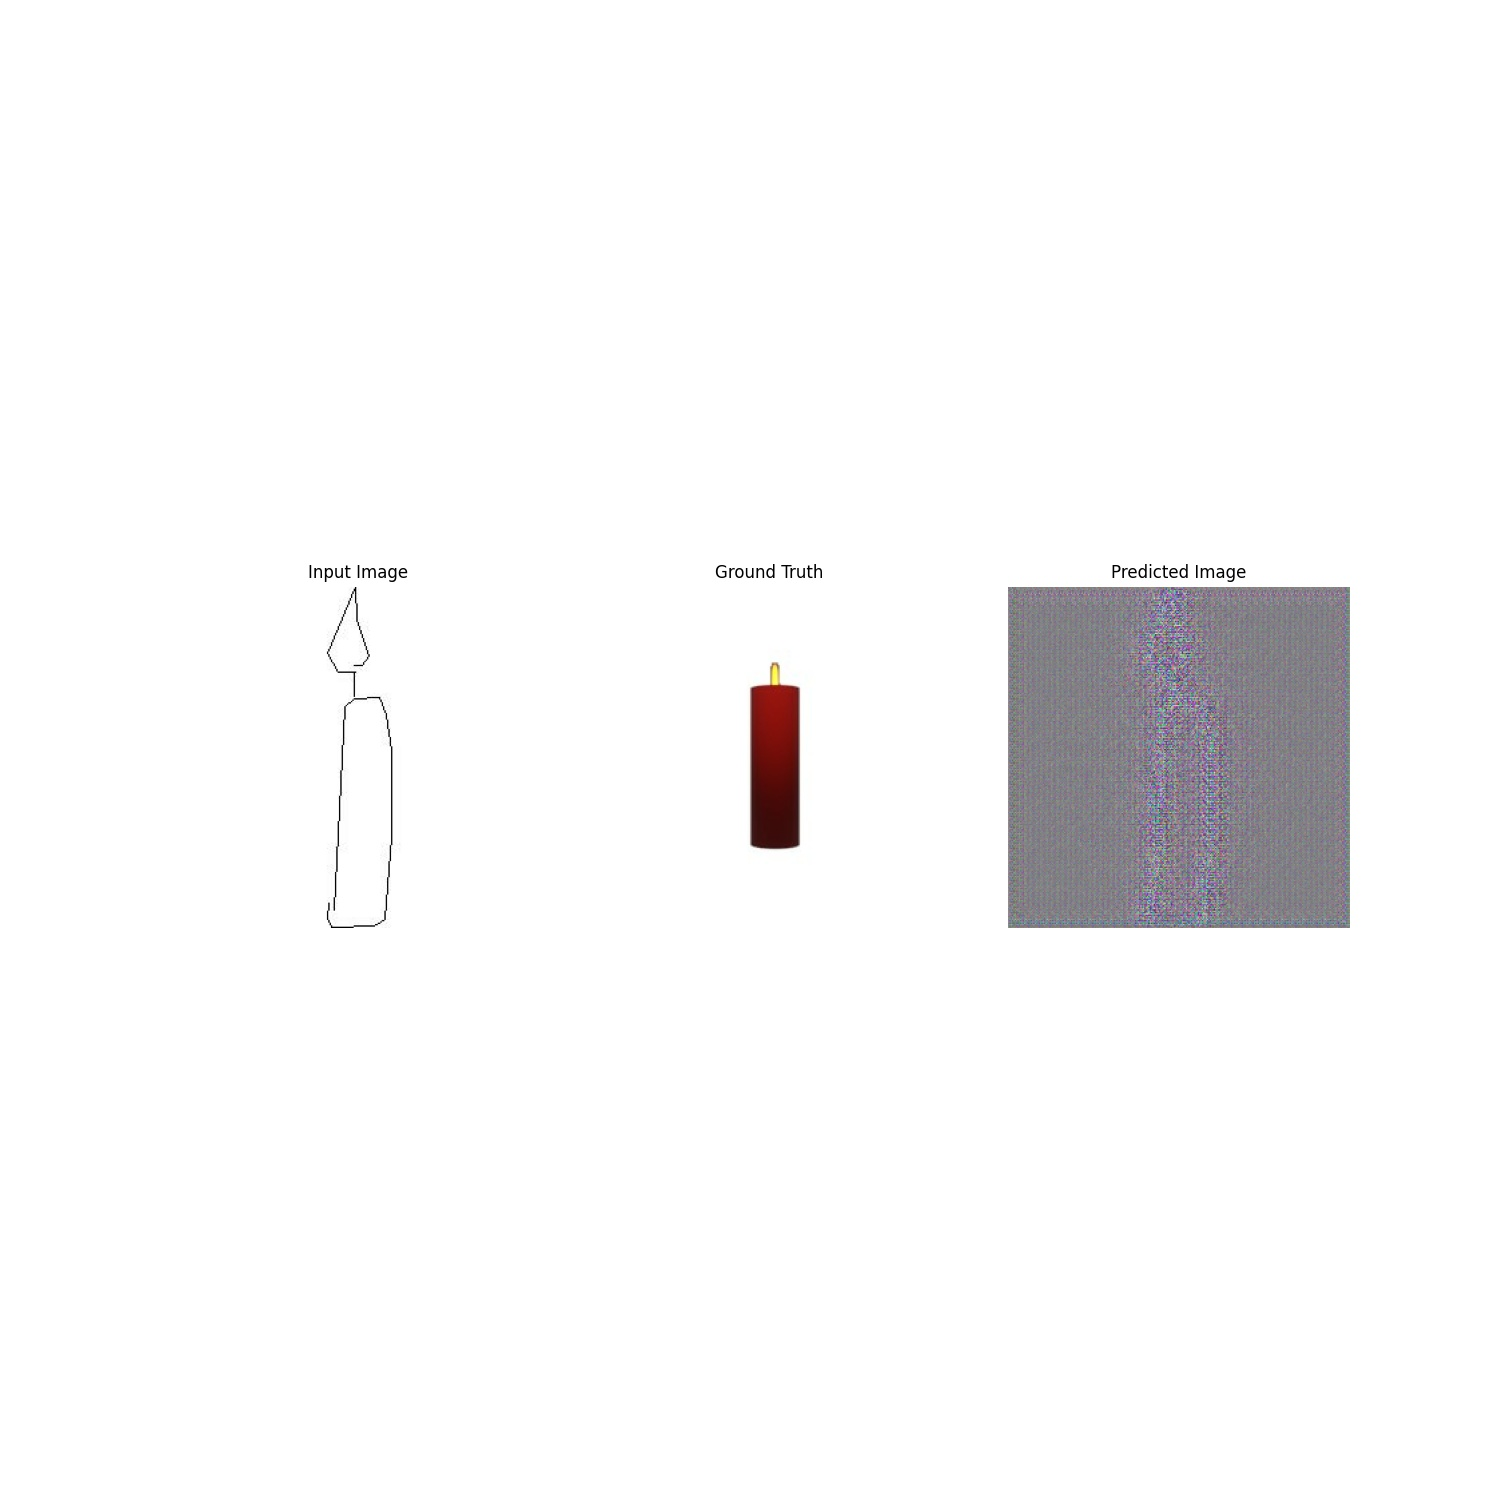
\includegraphics[width=0.3\textwidth]{bilder/0.jpg}
	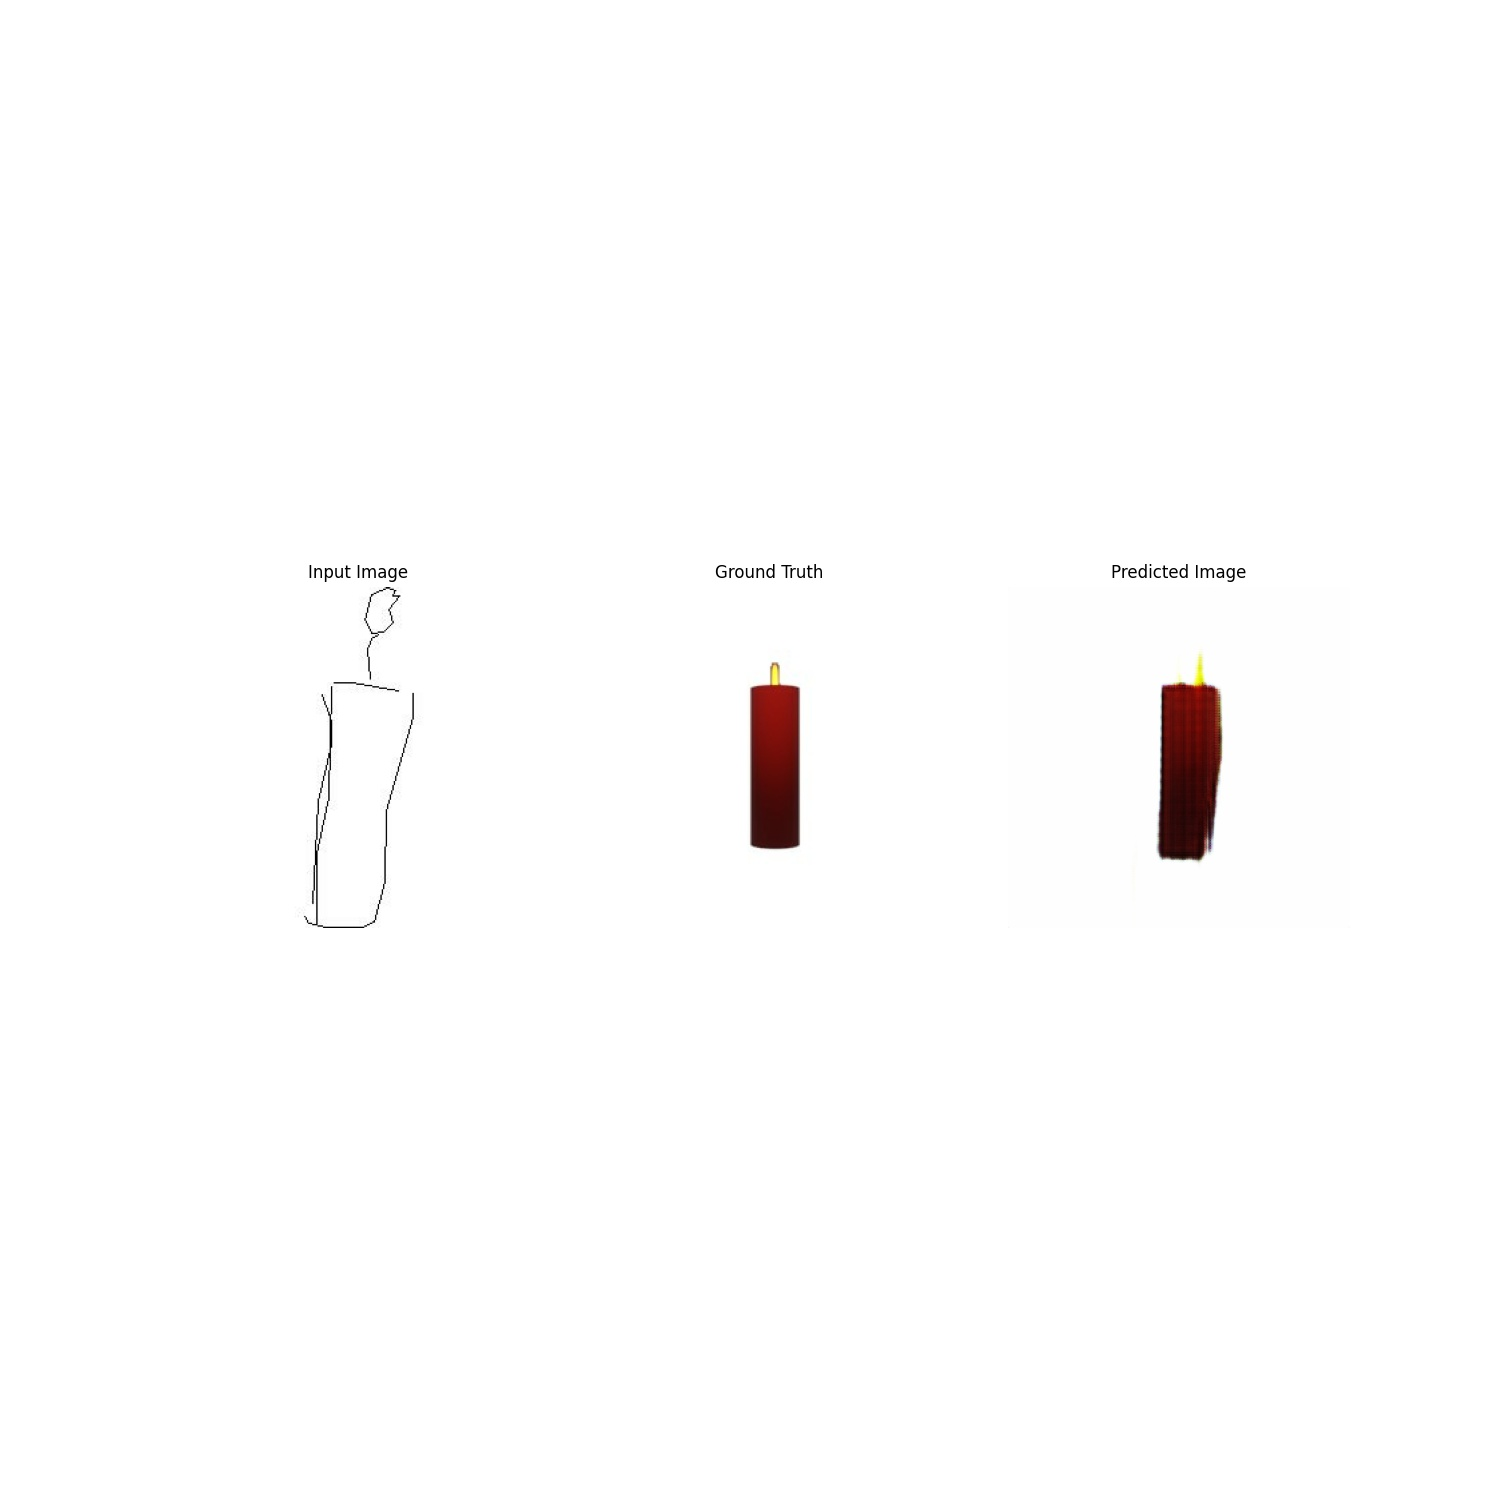
\includegraphics[width=0.3\textwidth]{bilder/1.jpg}
	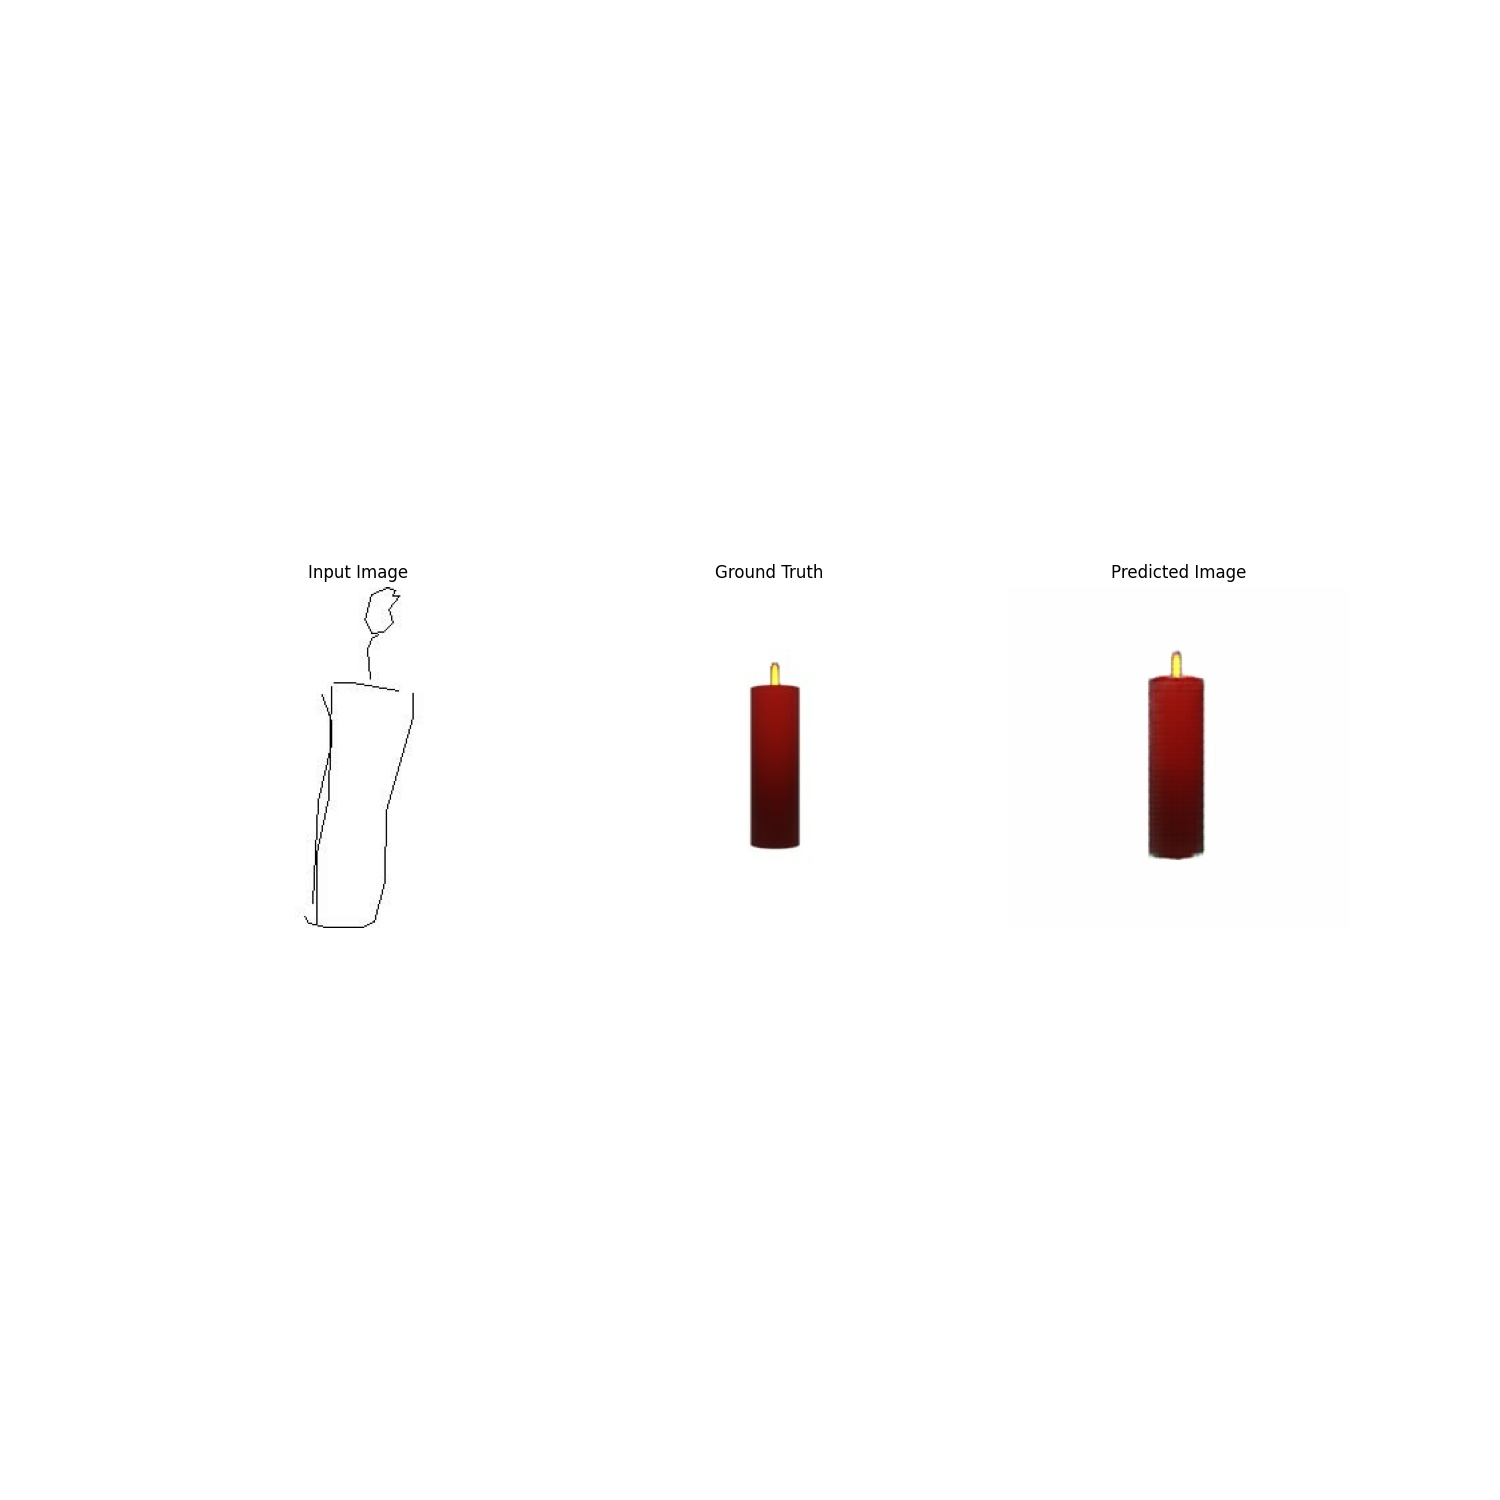
\includegraphics[width=0.3\textwidth]{bilder/15.jpg}
	\caption[Verschiedene Trainingsschritte]{Das Modell generiert das Ergebnis schrittweise aus zufälligem Rauschen. Nach 15000 Trainingsschritten ist das Ergebnis zufriedenstellend.}
	\label{fig:trichter}
\end{figure}

% Die Arbeit verfolgt das Ziel, verschiedene bewährte Architekturen künstlicher
% neuronaler Netze zur Generierung von Bildern zu untersuchen und in einem
% praxisorientierten Zusammenhang zu testen. Ich zeige mehrere Möglichkeiten,
% wirklichkeitsnahe Bilder von Alltagsgegenständen aus Skizzen, die durch Benutzer
% erstellt wurden, mittels eines künstlichen neuronalen Netzes zu generieren. Die
% Bilddateien der Skizzen sowie die generierten Bilddateien können dabei aus
% RBG-Pixelinformationen bestehen oder die Grafik mittels Bildkoordinaten beschreiben,
% wie es bei Vektorgrafiken und 3D-Modellen der Fall ist. Eine Anwendung der
% Ergebnisse ist beispielsweise als Feature eines Grafiktablets oder eines
% Smartboards denkbar.

\section{Bisherige Arbeiten}
\label{sec:related}
Künstliche neuronale Netze finden erst seit wenigen Jahren breite Aufmerksamkeit,
seit auch Heimcomputer in der Lage sind die hohe Anzahl der erforderlichen
Rechenoperationen in annehmbarer Zeit auszuführen. Seitdem sind wenige,
englischsprachige Einführungen in die Thematik entstanden. Ein häufig genanntes
Buch ist ``Deep Learning'', das online kostenfrei zugänglich ist \cite{Goodfellow-et-al-2016}.
Ebenfalls online kostenfrei ist das Buch ``Dive into Deep Learning'' \cite{zhang2020dive}.
Ein weiteres, praxisorientierteres Buch ist ``Deep Learning with Python'' \cite{chollet2021deep}, dessen
zweite Auflage bald herausgegeben wird.

Erste Recherchen haben verschiedene Arten und Implementierungen Bilder generierender künstlicher neuronaler Netze herausgestellt. Das Model aus ``DRAW: A Recurrent Neural Network For Image Generation'' \cite{gregor2015draw} kann darauf trainiert werden, handschriftliche Ziffern wie die des MNIST-Datasets zu generieren.

Die Schlüsselerkenntnis in ``A Neural Algorithm of Artistic Style'' \cite{gatys2015nst} ist, dass Inhalt und Stil eines Bildes voneinander getrennt werden können. Das Model kann zum Beispiel den Stil eines Künstlers auf das Bild eines anderen übertragen.

In anderen Ansätzen mit rekurrenten neuronalen Netzen wird jedes Eingabebild in eine Sequenz von Pixeln umgeformt. Anschließend wird das künstliche neuronale Netz darauf trainiert, teilweise geschwärzte Bilder wieder zu vervollständigen \cite{chen2020generative}, \cite{oord2016pixel}. Es werden auch Bilder generiert und die Fähigkeit des jeweiligen Models, die Darstellung von Bildern zu lernen, untersucht und mit der anderer Models verglichen. Ein weiterer, ebenfalls rekurrenter Algorithmus generiert Bilder aus textuellen Beschreibungen \cite{ramesh2021zeroshot}.

Besondere Aufmerksamkeit habe ich den Generative Adversarial Networks \cite{goodfellow2014generative} gegeben. Die Ergebnisse dieser Familie von künstlichen neuronalen Netzen sind teilweise erstaunlich gut, und es gibt bereits einige Beispielanwendungen und frei verfügbaren Quelltext. Je nach Anwendung des Models variiert die Qualität der Resultate.

Die vielseitigste Generierung von Bildern bietet Image-To-Image-Translation with Conditional Adversarial Networks \cite{isola2018imagetoimage}. In der Arbeit werden Labels in Fotos zurückübersetzt, Schwarzweißbilder coloriert und weitere Anwendungsbeispiele gezeigt. Vor allem die Übersetzung ``Kanten nach Foto'' (``Edges to Photo'') ist für mein Vorhaben relevant. Das Dokument enthält dafür mehrere Beispiele und Hinweise für die Anpassung der Hyperparameter. Der Algorithmus setzt auf Generative Adversarial Networks \cite{goodfellow2014generative} und Conditional Generative Adversarial Networks \cite{mirza2014conditional} auf.

In ``Unsupervised Representation Learning with Deep Convolutional Generative Adversarial Networks'' \cite{radford2016unsupervised} werden ebenfalls
realitätsnahe Ergebnisse erzielt. Anders als bei den bisher erwähnten Arbeiten
wird Unsupervised Learning verwendet, um das künstliche neuronale Netz zu trainieren.

\begin{figure}[h]
	\centering
	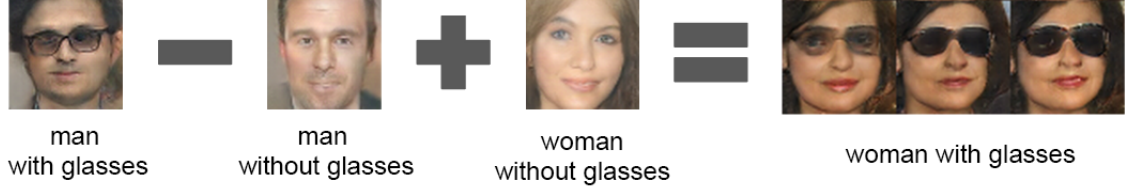
\includegraphics[width=1.0\textwidth]{bilder/image_arithmetic.png}
	\caption[Bildarithmetik]{Bildquelle: ``Unsupervised Representation Learning with Deep Convolutional Generative Adversarial Networks'' \cite{radford2016unsupervised} \newline Unter anderem werden dort Bilder in einer Art Arithmetik miteinander kombiniert, um ein neues Ergebnis zu erzeugen.}
	\label{fig:unsupervisedexamples}
\end{figure}

\begin{figure}[h]
	\centering
	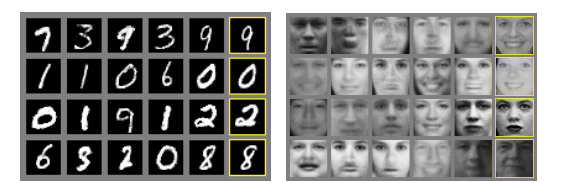
\includegraphics[width=1.0\textwidth]{bilder/mnist_faces.png}
	\caption[GAN Beispielbilder]{Bildquelle: ``Generative Adversarial Nets'' \cite{goodfellow2014generative} \newline Dieses Dokument zeigt mehrere Beispiele generierter Bilder. Es ist deutlich zu erkennen, wie gut der Algorithmus geeignet ist Bilder zu generieren. Die gelb gerahmten Bilder sind die Ground Truth aus dem jeweiligen Trainingsset.}
	\label{fig:ganexamples}
\end{figure}

\pagebreak

\begin{figure}[h]
	\centering
	\imagetranslation{bilder/edges2cats_a}{bilder/edges2cats_b}
	\hspace{.5cm}
	\imagetranslation{bilder/fotogenerator_a}{bilder/fotogenerator_b}
	\hspace{.5cm}
	\imagetranslation{bilder/sketch2portrait_a}{bilder/sketch2portrait_b}
	\label{fig:pix2pixexamples_1}
\end{figure}

\begin{figure}[h]
	\centering
	\imagetranslation{bilder/pokemon_a}{bilder/pokemon_b}
	\hspace{.5cm}
	\imagetranslation{bilder/shoe_a}{bilder/shoe_b}
	\hspace{.5cm}
	\imagetranslation{bilder/handbag_a}{bilder/handbag_b}
	\caption[Bildarithmetik]{Bildquelle: ``Image-To-Image-Translation with Conditional Adversarial Networks'' \cite{isola2018imagetoimage} \newline In dem Paper zu Pix2Pix sind viele Beispiele für die Generierung von Bildern aus Handzeichnungen oder Ergebnissen einer Kantenerkennung (zum Beispiel Canny Edge Detection) enthalten.}
	\label{fig:pix2pixexamples_2}
\end{figure}

\begin{figure}[h]
	\centering
	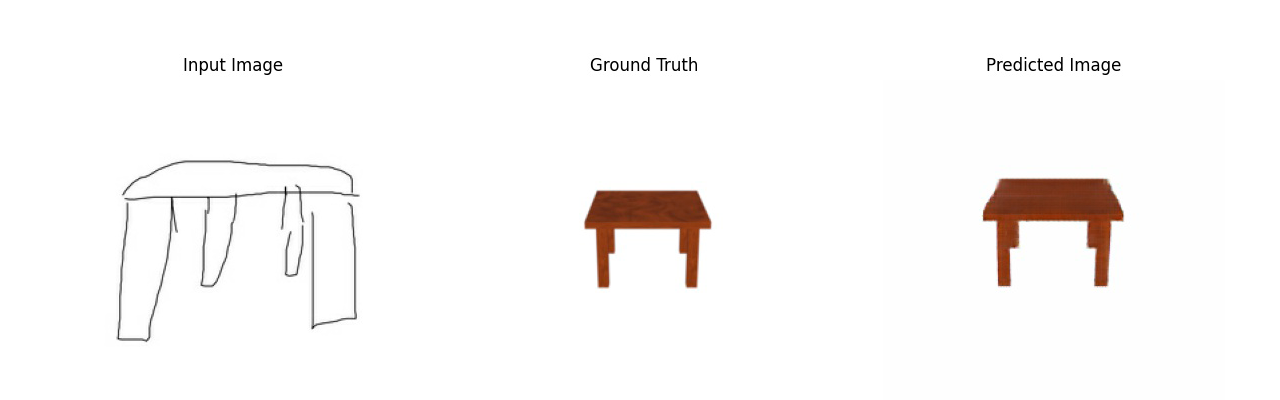
\includegraphics[width=0.6\textwidth]{bilder/table1small.png}
	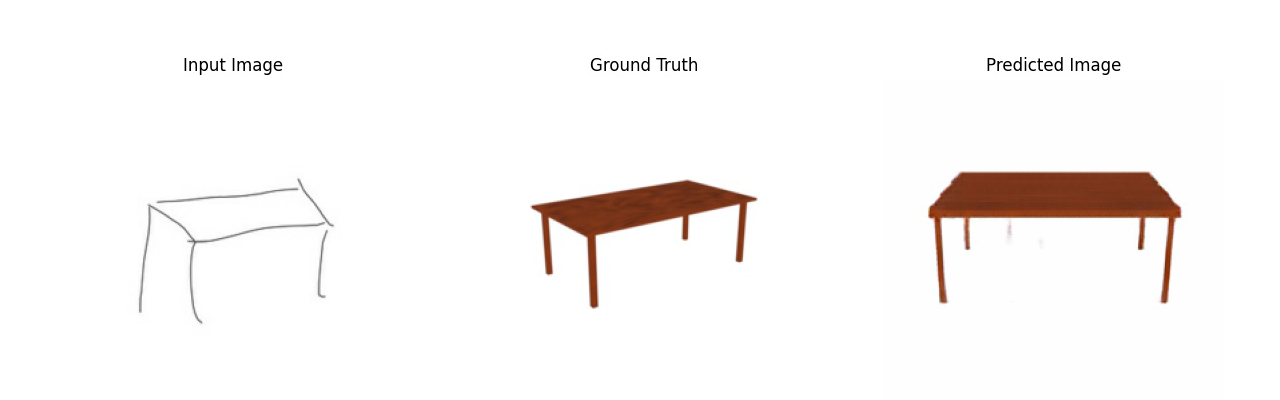
\includegraphics[width=0.6\textwidth]{bilder/table2small.png}
	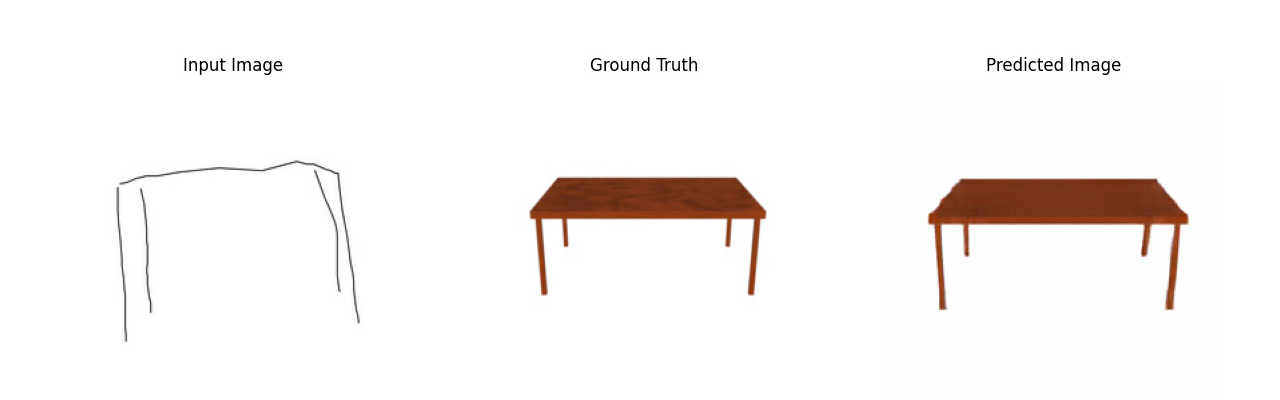
\includegraphics[width=0.6\textwidth]{bilder/table3small.png}

	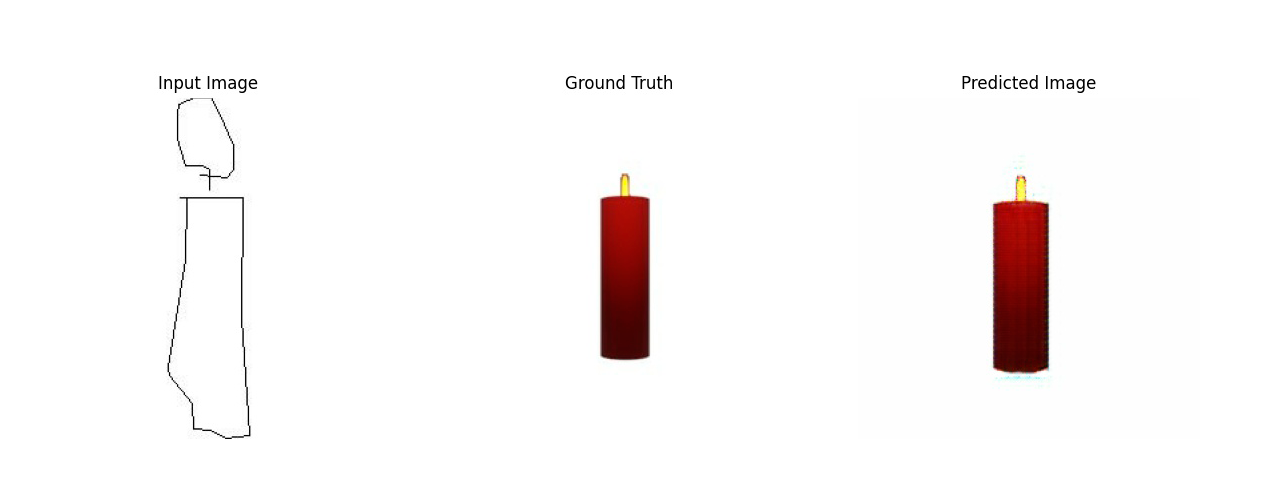
\includegraphics[width=0.6\textwidth]{bilder/candle1small.png}
	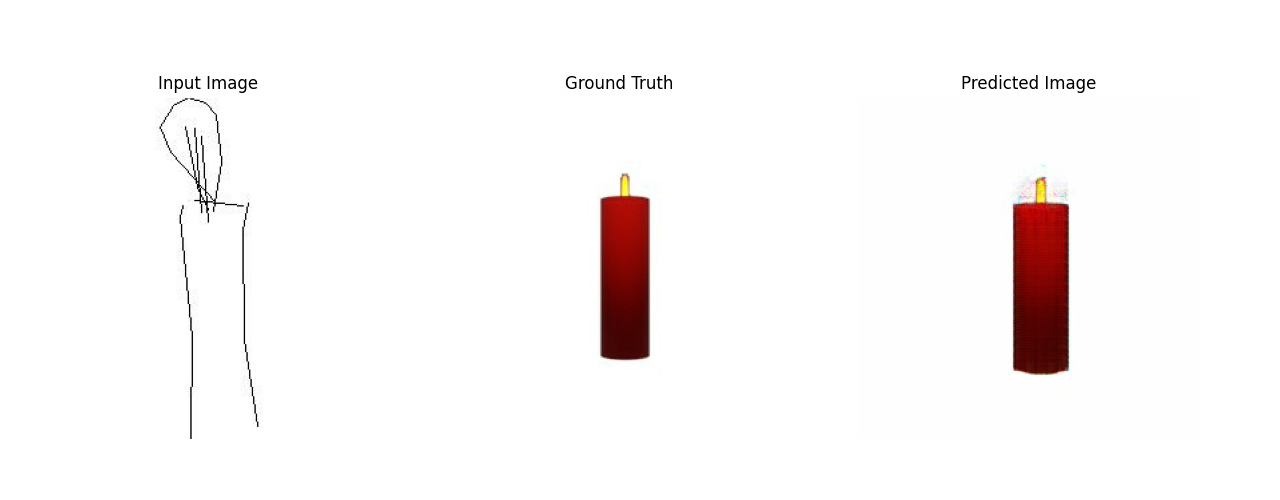
\includegraphics[width=0.6\textwidth]{bilder/candle2small.png}
	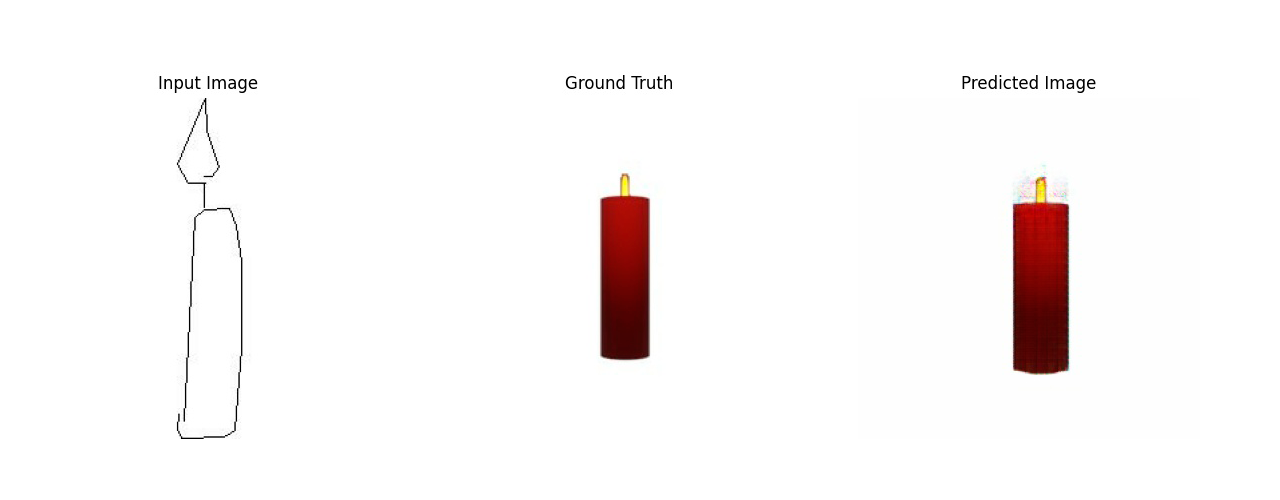
\includegraphics[width=0.6\textwidth]{bilder/candle3small.png}
	\caption[Eigene Beispiele]{Meine Ergebnisse zeigen, dass aus einer Handzeichnung ein fotorealistisches Bild generiert werden kann. Die generierten Bilder nehmen ungefähr die Proportionen der Handzeichnungen an, erstellen realistische Darstellungen der Gegengenstände und fügen Texturen und Lichteffekte hinzu.}
	\label{fig:myexamples}
\end{figure}

Blender ist ein 3D-Computergrafikprogramm mit Werkzeugen für die Modellierung und Animation von Objekten und Charakteren und zur Erstellung von Hintergrundszenen. Szenen können als Standbilder hergestellt werden. Animierte Sequenzen können für Videoproduktionen genutzt werden. Modelle und Szenen werden durch Farben und Texturen noch aufgewertet, wodurch brillante realistische Effekte produziert werden. Die Standbilder und Videos können als Kunstwerke oder als architektonisch oder wissenschaftliche Präsentationen Anwendung finden. \cite{blain2020blender}


\cleardoublepage
\chapter{Entwicklungsumgebung}
\label{ch:latex}

\section{Ubuntu Linux}
\label{sec:ubuntu}

\section{Python}
\label{sec:python}

\section{Tensorflow}
\label{sec:tensorflow}

\section{CUDA}
\label{sec:cuda}

\chapter{Neuronale Netze}
\label{ch:neuralnets}

\section{Logistic Regression}
\label{sec:logreg}

\section{Deep Neural Networks}
\label{sec:dnn}

\section{Convolutional Neural Networks}
\label{sec:cnn}

\section{Neural Style Transfer}
\label{sec:nst}


\chapter{Durchführung des Experiments}
\label{ch:conduct}

\section{Vorbereitung der Eingabedaten}
\label{sec:preparation}

\section{Anwendung herkömmlicher Shader}
\label{sec:shader}

\section{Hyperparameter}
\label{sec:hyperparams}

\section{Performancebeobachtungen}
\label{sec:performance}

\section{Zusammenfassung}
\label{sec:conclusion}


%weitere Kapitel hier einfügen

%\cleardoublepage
%\input{03_neues_kapitel}

%Literatur
\cleardoublepage
\printbibliography[heading=bibintoc]

%Bildnachweise
\cleardoublepage
\chapter*{Bildnachweis}
\addcontentsline{toc}{chapter}{Bildnachweis}

% \autoref{fig:trichter}: The Metropolitan Museum of Art,\\
% https://www.metmuseum.org/art/collection/search/202901, (CC0 1.0)

\autoref{fig:tensorboard}: {TensorFlow}: Large-Scale Machine Learning on Heterogeneous Systems,\\
https://www.tensorflow.org/, (CC BY 4.0 / Apache License 2.0) \\

\noindent
\autoref{fig:blender}: Blender Foundation,\\
https://www.blender.org/, (GNU GPLv3)

\noindent
\autoref{fig:pix2pixprogress3}: {TensorFlow}: Large-Scale Machine Learning on Heterogeneous Systems,\\
https://www.tensorflow.org/, (CC BY 4.0 / Apache License 2.0) \\

\noindent
\autoref{fig:pix2pixprogress4}: {TensorFlow}: Large-Scale Machine Learning on Heterogeneous Systems,\\
https://www.tensorflow.org/, (CC BY 4.0 / Apache License 2.0) \\

\noindent
TensorFlow, the TensorFlow logo and any related marks are trademarks of Google Inc.


%Abkürzungs- und Symbolverzeichnis
\cleardoublepage
\renewcommand{\chaptermark}[1]{\markboth{#1}{}}

\chapter*{Abkürzungs- und Symbolverzeichnis}
\addcontentsline{toc}{chapter}{Abkürzungs- und Symbolverzeichnis}
\label{ch:symbole_abk}
\chaptermark{Abkürzungs- und Symbolverzeichnis}

\noindent 
\textit{Abkürzungen}

\vspace{6pt}

\noindent 
\begin{tabular}{@{}p{2cm}l}
AC&Air Compressor, Luftverdichter\\
APH&Air Preheater, Luftvorwärmer\\
CC&Combustion Chamber, Brennkammer\\
EXP& Expander\\
HRSG&Heat Recovery Steam Generator, Abhitzekessel\\
\end{tabular}

%\clearpage

%\noindent
%\begin{tabular}{@{}p{2cm}l}
%IEA& International Energy Agency\\
%NASA& National Aeronautics \& Space Administration\\
%\end{tabular}

\vspace{18pt}
%\clearpage

\noindent 
\textit{Lateinische Symbole}

\vspace{6pt}

\noindent 
\begin{tabular}{@{}p{2cm}l}
	$c$&Spezifische Kosten je Exergieeinheit, \euro/J\textsubscript{ex}\\
	$\dot C$&Kostenstrom, \euro/h \\
	$CC$&Kapitalgebundene Kosten, \euro \\
	$c\!f$&Capacity Factor, Jährliche Auslastung, --\\	
	$e$&Spezifische Exergie, J/kg\\
	$\bar{e}$&Spezifisch molare Exergie, J/mol\\
	$\dot E$&Exergiestrom, W\\
	$f$&Exergoökonomischer Faktor, --\\
	$fc$&Spezifische Brennstoffkosten, \euro/J\\
	$FC$&Brennstoffkosten, \euro \\
	$h$&Spezifische Enthalpie, J/kg\\
	$\dot H$&Enthalpiestrom, W\\
	$HHV$&Brennwert, J/kg\\
\end{tabular}

\vspace{18pt}
%\clearpage

\noindent 
\textit{Griechische Symbole}

\vspace{6pt}

\noindent 
\begin{tabular}{@{}p{2cm}l}
	$\Delta$&Differenz\\
	$\varepsilon$&Exergetischer Wirkungsgrad, --\\
	$\eta_s$&Isentroper Wirkungsgrad, --\\
	$\kappa$&Isentropenexponenten, --\\
	$\lambda$&Luftzahl, --\\
\end{tabular}

\vspace{18pt}
%\clearpage

\noindent 
\textit{Hoch- und tiefgestelle Indizes}

\vspace{6pt}

\noindent 
\begin{tabular}{@{}p{2cm}l}
	0&Referenzpunkt, Thermodynamische Umgebung\\
	a&Avarage, Mittlere\\
	D&Destruction, Vernichtung\\
	F&Fuel, Brennstoff, Aufwand\\
	net&Netto\\
\end{tabular}


%Abbildungsverzeichnis
\cleardoublepage
\addcontentsline{toc}{chapter}{\listfigurename}
\listoffigures

%Tabellenverzeichnis
\cleardoublepage
\addcontentsline{toc}{chapter}{\listtablename}
\listoftables

%Anhang
\cleardoublepage
\appendix
\addtocontents{toc}{\protect\newpage}
\part*{Anhang}
\addcontentsline{toc}{chapter}{Anhang}

\chapter{Quelltexte}
\label{ch:a_sim}

\section{Image-To-Image-Translation main.py}
\label{pix2pixpy}

\begin{lstlisting}
import tensorflow as tf

import os
import time
import datetime

from matplotlib import pyplot as plt
from IPython import display

from tensorflow.compat.v1 import ConfigProto
from tensorflow.compat.v1 import InteractiveSession


def load(image_file):
    # Read and decode an image file to a uint8 tensor
    image = tf.io.read_file(image_file)
    image = tf.image.decode_jpeg(image)

    # Split each image tensor into two tensors:
    w = tf.shape(image)[1]
    w = w // 2
    input_image = image[:, :w, :]
    real_image = image[:, w:, :]

    # Convert both images to float32 tensors
    input_image = tf.cast(input_image, tf.float32)
    real_image = tf.cast(real_image, tf.float32)

    return input_image, real_image


def resize(input_image, real_image, height, width):
    input_image = tf.image.resize(
      input_image, [height, width], method=tf.image.ResizeMethod.NEAREST_NEIGHBOR)
    real_image = tf.image.resize(
      real_image, [height, width], method=tf.image.ResizeMethod.NEAREST_NEIGHBOR)

    return input_image, real_image


def random_crop(input_image, real_image):
    stacked_image = tf.stack([input_image, real_image], axis=0)
    cropped_image = tf.image.random_crop(
      stacked_image, size=[2, IMG_HEIGHT, IMG_WIDTH, 3]
    )

    return cropped_image[0], cropped_image[1]
\end{lstlisting}
\pagebreak
\begin{lstlisting}
# Normalizing the images to [-1, 1]
def normalize(input_image, real_image):
    input_image = (input_image / 127.5) - 1
    real_image = (real_image / 127.5) - 1

    return input_image, real_image


@tf.function()
def random_jitter(input_image, real_image):
    # Resizing to 286x286
    input_image, real_image = resize(input_image, real_image, 286, 286)

    # Random cropping back to 256x256
    input_image, real_image = random_crop(input_image, real_image)

    if tf.random.uniform(()) > 0.5:
        # Random mirroring
        input_image = tf.image.flip_left_right(input_image)
        real_image = tf.image.flip_left_right(real_image)

    return input_image, real_image


def load_image_train(image_file):
    input_image, real_image = load(image_file)
    input_image, real_image = random_jitter(input_image, real_image)
    input_image, real_image = normalize(input_image, real_image)

    return input_image, real_image


def load_image_test(image_file):
    input_image, real_image = load(image_file)
    input_image, real_image = resize(
      input_image, real_image, IMG_HEIGHT, IMG_WIDTH
    )
    input_image, real_image = normalize(input_image, real_image)

    return input_image, real_image


def downsample(filters, size, apply_batchnorm=True):
    initializer = tf.random_normal_initializer(0., 0.02)

    result = tf.keras.Sequential()
    result.add(
      tf.keras.layers.Conv2D(
        filters,
        size,
        strides=2,
        padding='same',
        kernel_initializer=initializer,
        use_bias=False
      )
    )

    if apply_batchnorm:
        result.add(tf.keras.layers.BatchNormalization())

    result.add(tf.keras.layers.LeakyReLU())

    return result

\end{lstlisting}
\pagebreak
\begin{lstlisting}
def upsample(filters, size, apply_dropout=False):
    initializer = tf.random_normal_initializer(0., 0.02)

    result = tf.keras.Sequential()
    result.add(
        tf.keras.layers.Conv2DTranspose(
            filters, size, strides=2,
            padding='same',
            kernel_initializer=initializer,
            use_bias=False
        )
    )

    result.add(tf.keras.layers.BatchNormalization())

    if apply_dropout:
        result.add(tf.keras.layers.Dropout(0.5))

    result.add(tf.keras.layers.ReLU())

    return result


def build_generator():
    inputs = tf.keras.layers.Input(shape=[256, 256, 3])

    down_stack = [
        downsample(64, 4, apply_batchnorm=False),  # (batch_size, 128, 128, 64)
        downsample(128, 4),  # (batch_size, 64, 64, 128)
        downsample(256, 4),  # (batch_size, 32, 32, 256)
        downsample(512, 4),  # (batch_size, 16, 16, 512)
        downsample(512, 4),  # (batch_size, 8, 8, 512)
        downsample(512, 4),  # (batch_size, 4, 4, 512)
        downsample(512, 4),  # (batch_size, 2, 2, 512)
        downsample(512, 4),  # (batch_size, 1, 1, 512)
    ]

    up_stack = [
        upsample(512, 4, apply_dropout=True),  # (batch_size, 2, 2, 1024)
        upsample(512, 4, apply_dropout=True),  # (batch_size, 4, 4, 1024)
        upsample(512, 4, apply_dropout=True),  # (batch_size, 8, 8, 1024)
        upsample(512, 4),  # (batch_size, 16, 16, 1024)
        upsample(256, 4),  # (batch_size, 32, 32, 512)
        upsample(128, 4),  # (batch_size, 64, 64, 256)
        upsample(64, 4),  # (batch_size, 128, 128, 128)
    ]

    initializer = tf.random_normal_initializer(0., 0.02)
    last = tf.keras.layers.Conv2DTranspose(
        OUTPUT_CHANNELS,
        4,
        strides=2,
        padding='same',
        kernel_initializer=initializer,
        activation='tanh'
    )  # (batch_size, 256, 256, 3)

    x = inputs

    # Downsampling through the model
    skips = []
    for down in down_stack:
        x = down(x)
        skips.append(x)

    skips = reversed(skips[:-1])

\end{lstlisting}
\pagebreak
\begin{lstlisting}
    # Upsampling and establishing the skip connections
    for up, skip in zip(up_stack, skips):
        x = up(x)
        x = tf.keras.layers.Concatenate()([x, skip])

    x = last(x)
    return tf.keras.Model(inputs=inputs, outputs=x)


def generator_loss(disc_generated_output, gen_output, target):
    gan_loss = loss_object(tf.ones_like(disc_generated_output), disc_generated_output)

    # Mean absolute error
    l1_loss = tf.reduce_mean(tf.abs(target - gen_output))

    total_gen_loss = gan_loss + (LAMBDA * l1_loss)

    return total_gen_loss, gan_loss, l1_loss


def build_discriminator():
    initializer = tf.random_normal_initializer(0., 0.02)

    inp = tf.keras.layers.Input(shape=[256, 256, 3], name='input_image')
    tar = tf.keras.layers.Input(shape=[256, 256, 3], name='target_image')

    x = tf.keras.layers.concatenate([inp, tar])  # (batch_size, 256, 256, channels*2)

    down1 = downsample(64, 4, False)(x)  # (batch_size, 128, 128, 64)
    down2 = downsample(128, 4)(down1)  # (batch_size, 64, 64, 128)
    down3 = downsample(256, 4)(down2)  # (batch_size, 32, 32, 256)

    zero_pad1 = tf.keras.layers.ZeroPadding2D()(down3)  # (batch_size, 34, 34, 256)
    conv = tf.keras.layers.Conv2D(
        512,
        4,
        strides=1,
        kernel_initializer=initializer,
        use_bias=False
    )(zero_pad1)  # (batch_size, 31, 31, 512)

    batchnorm1 = tf.keras.layers.BatchNormalization()(conv)

    leaky_relu = tf.keras.layers.LeakyReLU()(batchnorm1)

    zero_pad2 = tf.keras.layers.ZeroPadding2D()(leaky_relu)  # (batch_size, 33, 33, 512)

    last = tf.keras.layers.Conv2D(
        1, 4, strides=1, kernel_initializer=initializer
    )(zero_pad2)  # (batch_size, 30, 30, 1)

    return tf.keras.Model(inputs=[inp, tar], outputs=last)


def discriminator_loss(disc_real_output, disc_generated_output):
    real_loss = loss_object(tf.ones_like(disc_real_output), disc_real_output)

    generated_loss = loss_object(tf.zeros_like(disc_generated_output), disc_generated_output)

    total_disc_loss = real_loss + generated_loss

    return total_disc_loss


def generate_images(model, test_input, tar, image_index):
    prediction = model(test_input, training=True)
    plt.figure(figsize=(15, 15))

    display_list = [test_input[0], tar[0], prediction[0]]
    title = ['Input Image', 'Ground Truth', 'Predicted Image']

    for i in range(3):
        plt.subplot(1, 3, i + 1)
        plt.title(title[i])
        # Getting the pixel values in the [0, 1] range to plot.
        plt.imshow(display_list[i] * 0.5 + 0.5)
        plt.axis('off')

    plt.savefig('results/' + str(image_index) + '.jpg')


@tf.function
def train_step(input_image, target, step):
    with tf.GradientTape() as gen_tape, tf.GradientTape() as disc_tape:
        gen_output = generator(input_image, training=True)

        disc_real_output = discriminator([input_image, target], training=True)
        disc_generated_output = discriminator([input_image, gen_output], training=True)

        gen_total_loss, gen_gan_loss, gen_l1_loss =
            generator_loss(disc_generated_output, gen_output, target)
        disc_loss = discriminator_loss(disc_real_output, disc_generated_output)

    generator_gradients = gen_tape.gradient(
        gen_total_loss, generator.trainable_variables
    )
    discriminator_gradients = disc_tape.gradient(
        disc_loss, discriminator.trainable_variables
    )

    generator_optimizer.apply_gradients(
        zip(generator_gradients, generator.trainable_variables)
    )
    discriminator_optimizer.apply_gradients(
        zip(discriminator_gradients, discriminator.trainable_variables)
    )

    with summary_writer.as_default():
        tf.summary.scalar('gen_total_loss', gen_total_loss, step=step // 1000)
        tf.summary.scalar('gen_gan_loss', gen_gan_loss, step=step // 1000)
        tf.summary.scalar('gen_l1_loss', gen_l1_loss, step=step // 1000)
        tf.summary.scalar('disc_loss', disc_loss, step=step // 1000)


def fit(train_ds, test_ds, steps):
    example_input, example_target = next(iter(test_ds.take(1)))
    start = time.time()

    for step, (input_image, target) in train_ds.repeat().take(steps).enumerate():
        if step % 1000 == 0:
            display.clear_output(wait=True)

            if step != 0:
                print(f'Time taken for 1000 steps: {time.time() - start:.2f} sec\n')

            start = time.time()

            generate_images(generator, example_input, example_target, step.numpy() // 1000)
            print(f"Step: {step // 1000}k")

        train_step(input_image, target, step)

        # Training step
        if (step + 1) % 10 == 0:
            print('.', end='', flush=True)

        # Save (checkpoint) the model every 5k steps
        if (step + 1) % 5000 == 0:
            checkpoint.save(file_prefix=checkpoint_prefix)


if __name__ == '__main__':
    config = ConfigProto()
    config.gpu_options.allow_growth = True
    session = InteractiveSession(config=config)

    # Adjust this value to the number of training images
    BUFFER_SIZE = 400

    # The batch size of 1 produced better results
    # for the U-Net in the original pix2pix experiment
    BATCH_SIZE = 1

    # Each image is 256x256 in size
    IMG_WIDTH = 256
    IMG_HEIGHT = 256

    PATH = '../PIX2PIX/images/combined/candles/'
    train_dataset = tf.data.Dataset.list_files(PATH + 'train/*.png')
    train_dataset = train_dataset.map(
      load_image_train, num_parallel_calls=tf.data.AUTOTUNE
    )
    train_dataset = train_dataset.shuffle(BUFFER_SIZE)
    train_dataset = train_dataset.batch(BATCH_SIZE)

    try:
        test_dataset = tf.data.Dataset.list_files(str(PATH + 'test/*.png'))
    except tf.errors.InvalidArgumentError:
        test_dataset = tf.data.Dataset.list_files(str(PATH + 'val/*.png'))
    test_dataset = test_dataset.map(load_image_test)
    test_dataset = test_dataset.batch(BATCH_SIZE)

    OUTPUT_CHANNELS = 3

    generator = build_generator()

    LAMBDA = 100

    loss_object = tf.keras.losses.BinaryCrossentropy(from_logits=True)

    discriminator = build_discriminator()

    generator_optimizer = tf.keras.optimizers.Adam(2e-4, beta_1=0.5)
    discriminator_optimizer = tf.keras.optimizers.Adam(2e-4, beta_1=0.5)

    checkpoint_dir = './training_checkpoints'
    checkpoint_prefix = os.path.join(checkpoint_dir, "ckpt")
    checkpoint = tf.train.Checkpoint(
        generator_optimizer=generator_optimizer,
        discriminator_optimizer=discriminator_optimizer,
        generator=generator,
        discriminator=discriminator
    )

    log_dir = "logs/"

    summary_writer = tf.summary.create_file_writer(
        log_dir + "fit/" + datetime.datetime.now().strftime("%Y%m%d-%H%M%S")
    )

    fit(train_dataset, test_dataset, steps=40000)

\end{lstlisting}
\pagebreak
\begin{lstlisting}
    # Restoring the latest checkpoint in checkpoint_dir
    checkpoint.restore(tf.train.latest_checkpoint(checkpoint_dir))

    # Run the trained model on a few examples from the test set
    index = 1000
    for inp, tar in test_dataset.take(5):
        generate_images(generator, inp, tar, index)
        index = index + 1

\end{lstlisting}
\vfill

\pagebreak

\section{Python-Script zur Generierung von JPEG-Bilddateien aus NDJSON-Informationen}
\label{ndjsonpy}

\begin{lstlisting}
import os
from functools import reduce
import tensorflow as tf
import json
from PIL import Image, ImageDraw

MAX_JPGS = 5000

dataset = tf.data.TextLineDataset(['../full_simplified_car.ndjson'])

for index, line in enumerate(dataset):
    if index % 1000 == 0:
        print(f'{index} of {MAX_JPGS}')
    jsonLine = json.loads(line.numpy())
    drawing = jsonLine['drawing']

    im = Image.new('RGB', (256, 256), (255, 255, 255))
    draw = ImageDraw.Draw(im)

    # normalise coords to center the drawing
    x_coords = reduce(lambda a, b: a + b, [stroke[0] for stroke in drawing])
    displacement_x = int((256 - min(x_coords) - max(x_coords)) / 2)
    y_coords = reduce(lambda a, b: a + b, [stroke[1] for stroke in drawing])
    displacement_y = int((256 - min(y_coords) - max(y_coords)) / 2)

    for stroke in drawing:
        draw.line(list(zip(
          [x + displacement_x for x in stroke[0]],
          [y + displacement_y for y in stroke[1]]
        )), fill=0)

    im.save(os.path.join('cars', str(index) + '.jpg'), 'JPEG')

    with open(os.path.join('json', str(index) + '.json'), 'w') as file:
        file.write(json.dumps(drawing))

    if index == MAX_JPGS:
        break
\end{lstlisting}
\vfill

\pagebreak

\section{Blender-Python-Script zur Generierung von Tischen}
\label{blenderpy}

\begin{lstlisting}
import bpy
import math
import random

obj_filepath = '/home/sberger/blender/tables/obj/random_table{}.obj'
render_filepath = '/home/sberger/blender/tables/rendered/random_table{}_render{}.jpg'

for tableIndex in range(0, 50):
    # add table top
    tableWidth = random.random() * 8 + 6
    tableHeight = random.random() * .5 + .1
    tableDepth = random.random() * 4 + 4
    legLength = random.random() * 4 + 1
    bpy.ops.mesh.primitive_cube_add(
      size=1, enter_editmode=False, location=(0, tableHeight / 2 + legLength, 0)
    )
    bpy.context.object.name = 'Table'
    bpy.ops.transform.resize(
      value=(tableWidth, tableHeight, tableDepth),
      orient_type='GLOBAL',
      orient_matrix=((1, 0, 0), (0, 1, 0), (0, 0, 1)),
      orient_matrix_type='GLOBAL',
      constraint_axis=(False, True, False),
      mirror=True, use_proportional_edit=False,
      proportional_edit_falloff='SMOOTH',
      proportional_size=1,
      use_proportional_connected=False,
      use_proportional_projected=False
    )
    bpy.context.active_object.data.materials.append(bpy.data.materials.get("Wood"))

    # add table legs
    legWidth = random.random() * .5 + .1
    legDisplacement = random.random() * 1 + legWidth / 2
    legDisplacementX = tableWidth / 2 - legDisplacement
    legDisplacementZ = tableDepth / 2 - legDisplacement

    for legIndex, coords in enumerate([
      [legDisplacementX, legDisplacementZ],
      [-legDisplacementX, legDisplacementZ],
      [legDisplacementX, -legDisplacementZ],
      [-legDisplacementX, -legDisplacementZ]
    ]):
        bpy.ops.mesh.primitive_cube_add(
          size=1, enter_editmode=False, location=(coords[0], legLength / 2, coords[1])
        )
        bpy.context.object.name = 'TableLeg' + str(legIndex)
        bpy.ops.transform.resize(
          value=(legWidth, legLength, legWidth),
          orient_type='GLOBAL',
          orient_matrix=((1, 0, 0), (0, 1, 0), (0, 0, 1)),
          orient_matrix_type='GLOBAL',
          constraint_axis=(False, True, False),
          mirror=True,
          use_proportional_edit=False,
          proportional_edit_falloff='SMOOTH',
          proportional_size=1,
          use_proportional_connected=False,
          use_proportional_projected=False
        )
        bpy.context.active_object.data.materials.append(bpy.data.materials.get("Wood"))

    # export to wavefront obj format
    bpy.ops.export_scene.obj(filepath = obj_filepath.format(tableIndex))

    # rotate and render
    bpy.ops.object.select_all(action='DESELECT')
    bpy.data.objects['Table'].select_set(True)
    for legIndex in range(0, 4):
        bpy.data.objects['TableLeg' + str(legIndex)].select_set(True)
    bpy.ops.object.transform_apply(location=False, rotation=True, scale=False)
    for renderIndex in range(0, 5):
        # rotate table
        bpy.ops.transform.rotate(
          value=math.pi / 5,
          orient_axis='Y',
          orient_type='GLOBAL',
          orient_matrix=((1, 0, 0), (0, 1, 0), (0, 0, 1)),
          orient_matrix_type='GLOBAL',
          constraint_axis=(False, True, False),
          mirror=True,
          use_proportional_edit=False,
          proportional_edit_falloff='SMOOTH',
          proportional_size=1,
          use_proportional_connected=False,
          use_proportional_projected=False
        )

        # render
        bpy.context.scene.render.filepath = render_filepath.format(tableIndex, renderIndex)
        bpy.ops.render.render(write_still = True)

    #delete objects
    bpy.ops.object.delete(use_global=False)
\end{lstlisting}


\end{document}
